\begin{frame}{Symulowane wyżarzanie [ang. \textit{Simulated Annealing}]}

	\begin{block}{}
	Rodzaj algorytmu heurystycznego przeszukującego przestrzeń alternatywnych rozwiązań problemu w celu wyszukiwania rozwiązań najlepszych. Jest wariantem metody przeszukiwania lokalnego [ang. \textit{Local Search}].
	Ogólny szkic działania algorytmu symulowanego wyżarzania:
	\end{block}
	\begin{enumerate}
		\item losowy wybór punktu startowego
		\item losowy wybór sąsiada
		\item odpowiednia akceptacja sąsiada
		\item po każdej iteracji temperatura zostaje zaktualizowana:
			$$ T = n\cdot T \wedge n \in (0,1)$$
		\item algorytm zatrzymuje się gdy w ciągu ustalonej liczby iteracji nie uda się osiągnąć lepszego wyniku
	\end{enumerate}

    \begin{block}{Wybór sąsiada}
        Parokrotne wykonanie transpozycji na rozpatrywanym osobiku.
    \end{block}
\end{frame}

\begin{frame}{Temeratura}
    \begin{equation}
        t(i, n) = 1 - e^\frac{1}{\frac{i}{n} - 1}
    \end{equation}

    \begin{description}
        \item[$i$] -- iteracja
        \item[$n$] -- maksymalna ilość iteracji
    \end{description}

    \begin{figure}
        \centering
        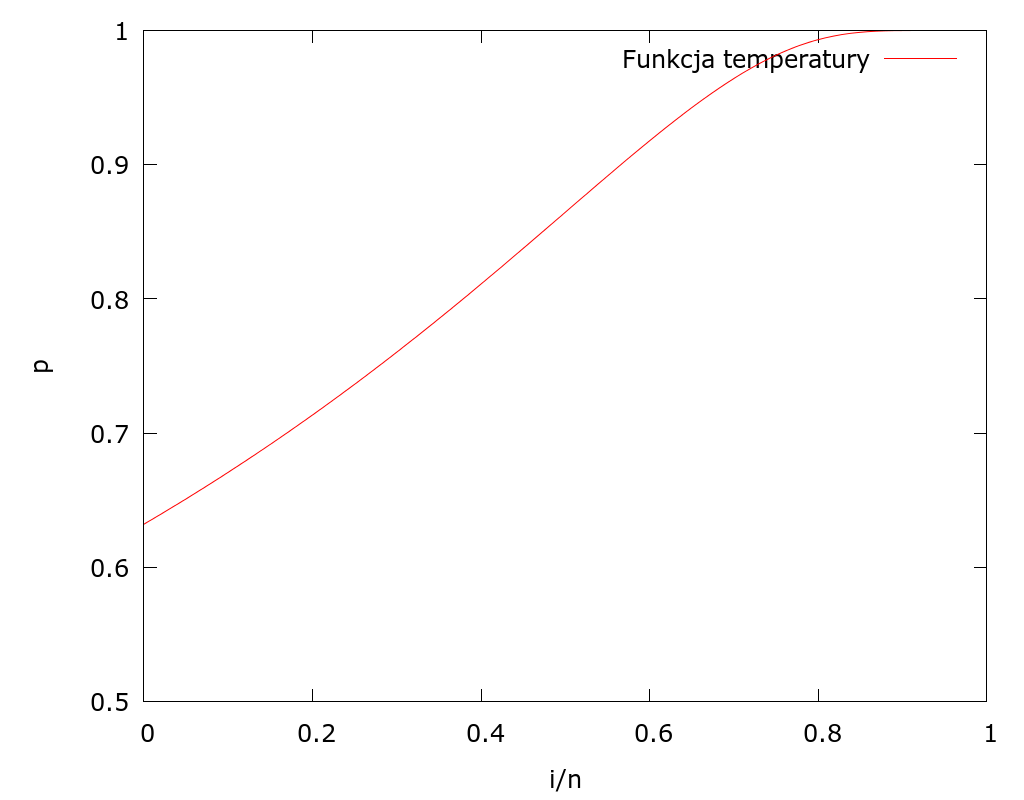
\includegraphics[width=5cm]{charts/temp.png}
        \caption{Wykres prawdopodobienstwa wyboru lepszego osobnika}
    \end{figure}
\end{frame}

%\begin{frame}{Symulowane wyżarzanie [ang. \textit{Simulated Annealing}]}
%
%    \begin{algorithmic}[H]
%    \State $n -- \ \text{dlugosc permutacji}$
%    \While{$k = 0 to n^2$}{
%    }
%    \end{algorithmic}
%	\scalebox{0.4}{
%	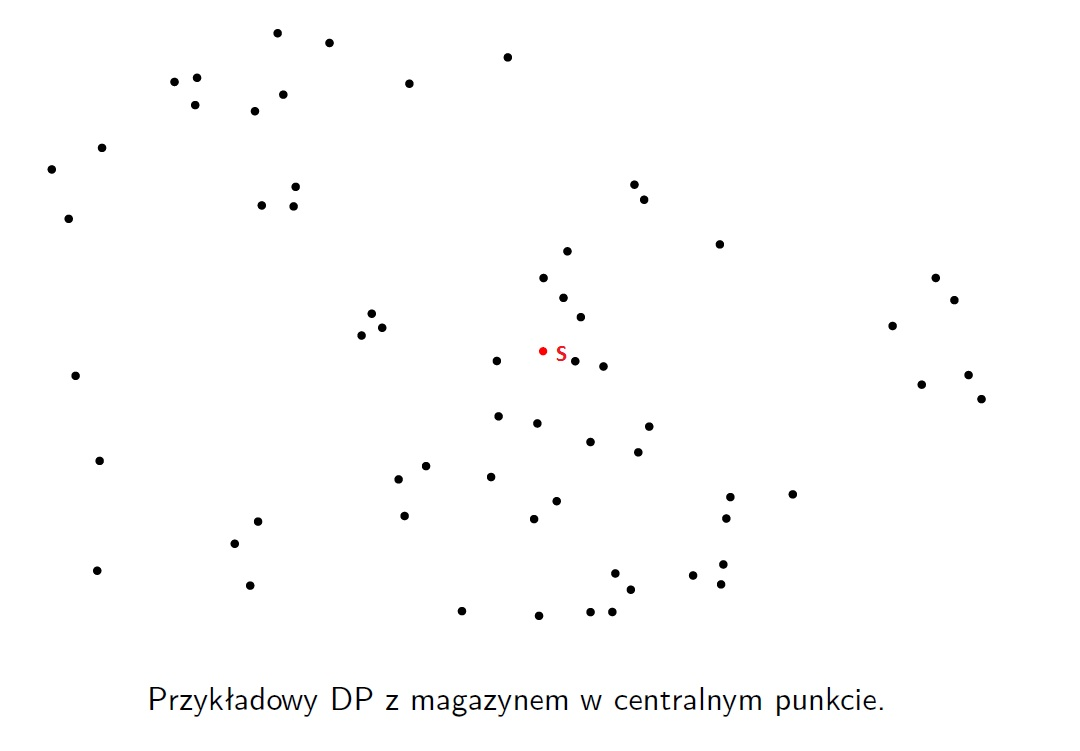
\includegraphics{./slajdy/1.jpg}}
%
%\end{frame}

%\begin{frame}{Symulowane wyżarzanie [ang. \textit{Simulated Annealing}]}
%
%	\scalebox{0.4}{
%	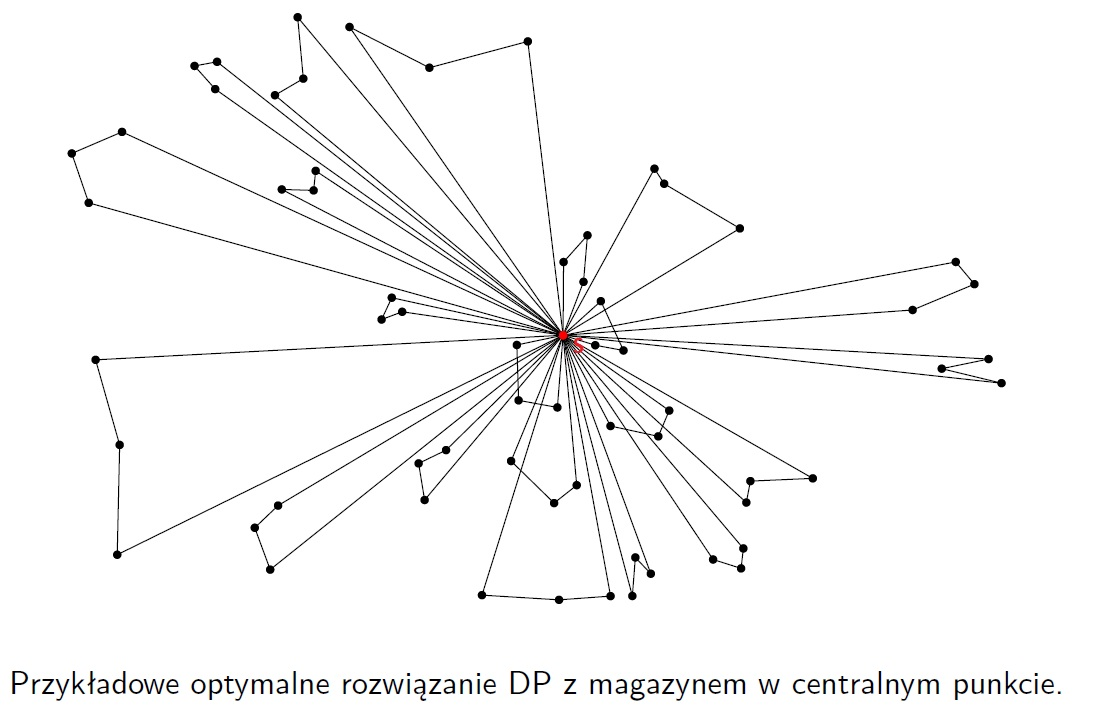
\includegraphics{./slajdy/2.jpg}}
%
%\end{frame}

%\begin{frame}{Symulowane wyżarzanie [ang. \textit{Simulated Annealing}]}
%	
%	\scalebox{0.4}{
%	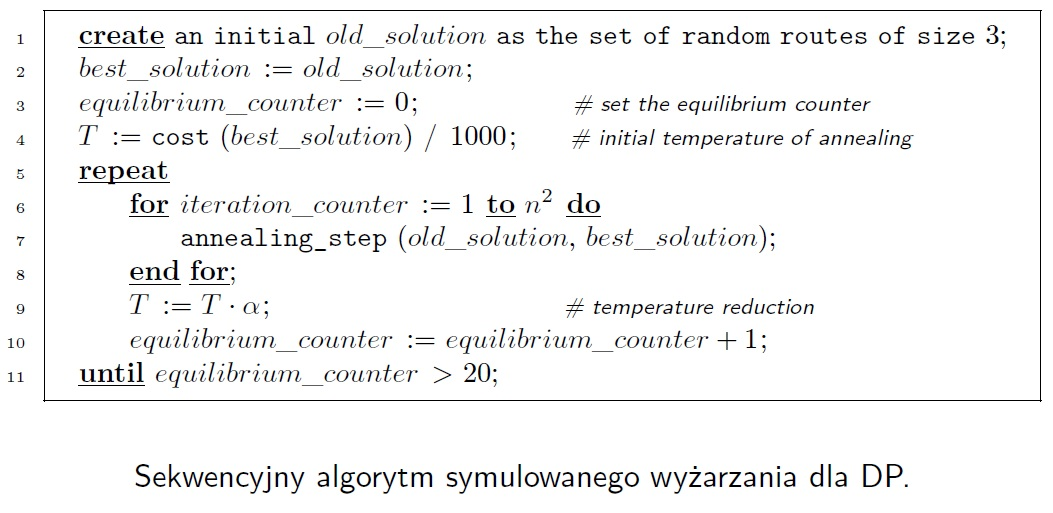
\includegraphics{./slajdy/3.jpg}}
%
%\end{frame}

%\begin{frame}{Symulowane wyżarzanie [ang. \textit{Simulated Annealing}]}
%
%	\scalebox{0.4}{
%	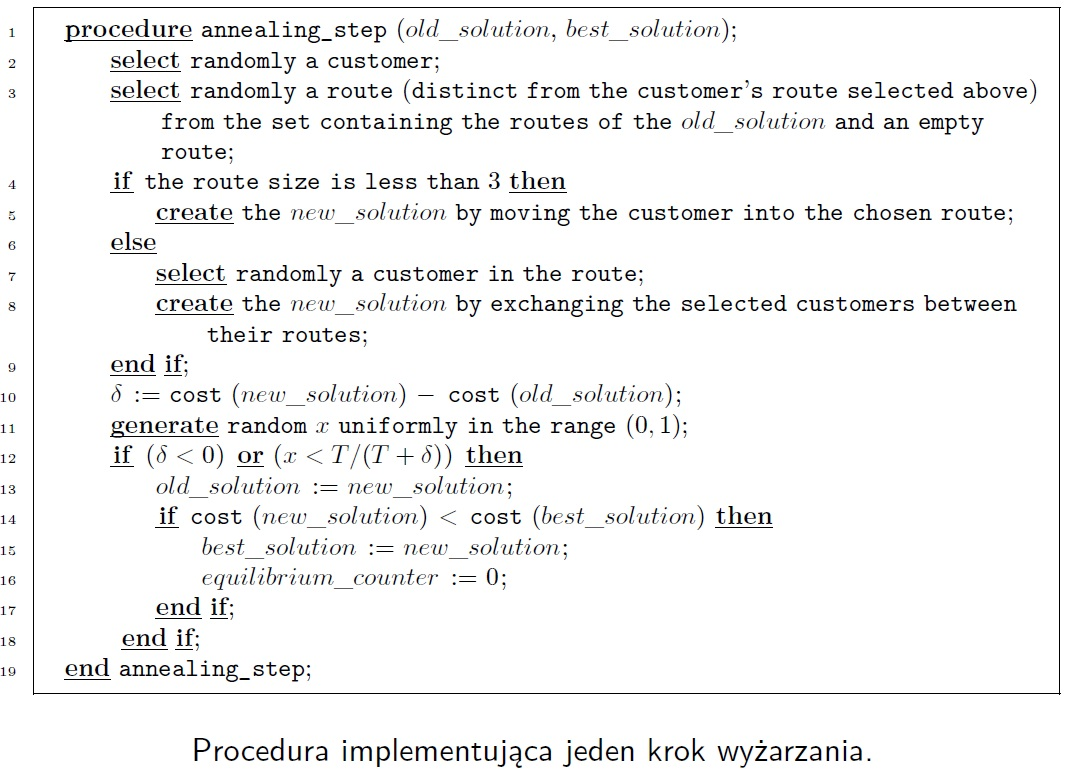
\includegraphics{./slajdy/4.jpg}}
%
%\end{frame}
